\documentclass[]{book}
\usepackage{lmodern}
\usepackage{amssymb,amsmath}
\usepackage{ifxetex,ifluatex}
\usepackage{fixltx2e} % provides \textsubscript
\ifnum 0\ifxetex 1\fi\ifluatex 1\fi=0 % if pdftex
  \usepackage[T1]{fontenc}
  \usepackage[utf8]{inputenc}
\else % if luatex or xelatex
  \ifxetex
    \usepackage{mathspec}
  \else
    \usepackage{fontspec}
  \fi
  \defaultfontfeatures{Ligatures=TeX,Scale=MatchLowercase}
\fi
% use upquote if available, for straight quotes in verbatim environments
\IfFileExists{upquote.sty}{\usepackage{upquote}}{}
% use microtype if available
\IfFileExists{microtype.sty}{%
\usepackage{microtype}
\UseMicrotypeSet[protrusion]{basicmath} % disable protrusion for tt fonts
}{}
\usepackage[margin=1in]{geometry}
\usepackage{hyperref}
\hypersetup{unicode=true,
            pdftitle={Crime Mapping and Spatial Analysis},
            pdfauthor={John Palmer},
            pdfborder={0 0 0},
            breaklinks=true}
\urlstyle{same}  % don't use monospace font for urls
\usepackage{natbib}
\bibliographystyle{apalike}
\usepackage{longtable,booktabs}
\usepackage{graphicx,grffile}
\makeatletter
\def\maxwidth{\ifdim\Gin@nat@width>\linewidth\linewidth\else\Gin@nat@width\fi}
\def\maxheight{\ifdim\Gin@nat@height>\textheight\textheight\else\Gin@nat@height\fi}
\makeatother
% Scale images if necessary, so that they will not overflow the page
% margins by default, and it is still possible to overwrite the defaults
% using explicit options in \includegraphics[width, height, ...]{}
\setkeys{Gin}{width=\maxwidth,height=\maxheight,keepaspectratio}
\IfFileExists{parskip.sty}{%
\usepackage{parskip}
}{% else
\setlength{\parindent}{0pt}
\setlength{\parskip}{6pt plus 2pt minus 1pt}
}
\setlength{\emergencystretch}{3em}  % prevent overfull lines
\providecommand{\tightlist}{%
  \setlength{\itemsep}{0pt}\setlength{\parskip}{0pt}}
\setcounter{secnumdepth}{5}
% Redefines (sub)paragraphs to behave more like sections
\ifx\paragraph\undefined\else
\let\oldparagraph\paragraph
\renewcommand{\paragraph}[1]{\oldparagraph{#1}\mbox{}}
\fi
\ifx\subparagraph\undefined\else
\let\oldsubparagraph\subparagraph
\renewcommand{\subparagraph}[1]{\oldsubparagraph{#1}\mbox{}}
\fi

%%% Use protect on footnotes to avoid problems with footnotes in titles
\let\rmarkdownfootnote\footnote%
\def\footnote{\protect\rmarkdownfootnote}

%%% Change title format to be more compact
\usepackage{titling}

% Create subtitle command for use in maketitle
\providecommand{\subtitle}[1]{
  \posttitle{
    \begin{center}\large#1\end{center}
    }
}

\setlength{\droptitle}{-2em}

  \title{Crime Mapping and Spatial Analysis}
    \pretitle{\vspace{\droptitle}\centering\huge}
  \posttitle{\par}
  \subtitle{Lab Manual}
  \author{John Palmer}
    \preauthor{\centering\large\emph}
  \postauthor{\par}
      \predate{\centering\large\emph}
  \postdate{\par}
    \date{2020-01-23}

\usepackage{booktabs}

\begin{document}
\maketitle

{
\setcounter{tocdepth}{1}
\tableofcontents
}
\hypertarget{cover}{%
\chapter*{Cover}\label{cover}}
\addcontentsline{toc}{chapter}{Cover}

\hypertarget{introduction}{%
\chapter*{Introduction}\label{introduction}}
\addcontentsline{toc}{chapter}{Introduction}

This manual is intended to function as a companion to the \emph{Crime Mapping and Spatial Analysis} labs as well as a stand-along reference for working with QGIS, Stata, and R for mapping and analysis. Each chapter walks you through a particular task or set of tasks, usually with an exercise to serve as an example. These are organized according to the class lab sessions but can also be followed intependently or used as a reference.

\hypertarget{accessing-qgis}{%
\section*{Accessing QGIS}\label{accessing-qgis}}
\addcontentsline{toc}{section}{Accessing QGIS}

QGIS is free and open source software, which you can download from \url{https://qgis.org}. At the time of writing, version 3.4 is the most recent long-term stable release and this manual is based on that version. When installing QGIS, leaving all of the default options as they are should be fine for purposes of this manual. The Windows installation includes a number of different choices for running QGIS; you shoud simply select the normal desktop version.

\hypertarget{accessing-stata}{%
\section*{Accessing Stata}\label{accessing-stata}}
\addcontentsline{toc}{section}{Accessing Stata}

Stata is proprietary software, which cannot be freely downloaded if have not purchased a license. However, as a UPF student, you have free access to Stata on the UPF lab computers and through UPF's \emph{MyApps} platform. The latter requires an internet connection and has some limitations in terms of resources, but you can access it from outside UPF using your own computer and a web browser.

To access Stata through \emph{MyApps}, open a web browser and go to \url{https://myapps.upf.edu}. Log in using your UPF user ID (uxxxxx) and the password you use for logging into UPF computers (i.e.~your birthdate, written as DDMMYYYY). Remember that this is not necessarily the password you use for Campus Global; your browser may have that Campus Global password stored, in which case you will need to manually change it each time. On the login page, you will need to choose between using \emph{vWorkspace Connector} or simply through your web browser with HTML5. The first option allows you to access local files on your computer, but it can be slow and ``buggy'', particularly on Macs. To follow this approach, click the \emph{Install} button on the page you reach after logging in. The second option can be faster, but any files you want to use will need to be first uploaded through the UPF MyCloud. To follow this approach, click the \emph{Continue} button on the page after login, and then flip the \emph{HTML5} switch to the on position at the top right of your screen.

\hypertarget{accessing-r}{%
\section*{Accessing R}\label{accessing-r}}
\addcontentsline{toc}{section}{Accessing R}

R is free and open source software, which you can download from \url{https://cran.r-project.org/}. You will normally want to install the latest release from that site, and to then install a good text editor or Integrated Development Environment (IDE). An excellent choice for the latter is the (free) Open Source Edition of RStudio, which you can download from \url{https://www.rstudio.com}. R and RStudio are also both available on the lab computers. This manual will assume that you are running RStudio.

\hypertarget{lab-instructions}{%
\chapter*{Lab Instructions}\label{lab-instructions}}
\addcontentsline{toc}{chapter}{Lab Instructions}

This section provides instructions for each lab session

\hypertarget{lab-1-9-january-2020}{%
\section*{Lab 1: 9 January 2020}\label{lab-1-9-january-2020}}
\addcontentsline{toc}{section}{Lab 1: 9 January 2020}

The core of criminology research involves observing the world around you, thinking about it, and communicating your thoughts to others. Computers can be useful tools for this, and most of the labs will focus on how to make use of them. Yet, computers can also get in the way. They can distort our observations and encourage us to think and communicate in certain ways. For this lab, therefore, we will start by actually going outside into the real world, making observations, and using a pen and paper to think about them and communicate them.

Your task for this lab is to observe the courtyard in the middle of the Jaume I building, think about the following questions, and draw a map to explain your thoughts to someone else:

\begin{itemize}
\tightlist
\item
  How many people are in the courtyard? Note, of course, that you will need to make some decision about time to answer this question: How many people right now? How many people over the course of an hour? Think about how the way you refine the question in this way will affect not just your answer but also the methods you use for reaching it.
\item
  Where are these people? In other words, how are these people you observe in the courtyard spatially distributed? (Again, time comes into play here, so we might be better off asking how they are spatio-temporally distributed.)
\item
  What are these people doing and where are they doing it? For example, are people reading, looking at their phones, talking, walking, running\ldots{}? Where are these activities taking place? For activities that involve movement, how can you best communicate how this movement is occurring?
\item
  What aspects of the physical environment (benches, walls, entry and exit points\ldots{}) seem to play an important role in the social activity you are observing?
\end{itemize}

We will proceed with this in several steps:

\begin{enumerate}
\def\labelenumi{\arabic{enumi}.}
\tightlist
\item
  Conduct an initial assessment of the courtyard and develop a strategy for answering the questions and communicating them on a map. You can do this in groups or on your own.
\item
  We will then reconvene as a class to discuss your strategies.
\item
  Now return to the courtyard and carry out your observations, analysis, and mapping. You can work in groups but you will each need to produce a set of maps that convey your findings. These maps should be drawn by hand.
\item
  We will then reconvene again to discuss your finished maps.
\item
  Finally, we will start using QGIS using the \emph{Getting Started with QGIS} section of this manual.
\end{enumerate}

At the end of the lab, you should hand in your hand-drawn maps. They will be evaluated based on your ideas, not based on how well you draw, how neat they are etc. The goal here is to get you to think through what how to communicate this information visually. How you then execute this technically, will form much of what we cover in the coming labs.

\hypertarget{lab-2-23-january-2020}{%
\section*{Lab 2: 23 January 2020}\label{lab-2-23-january-2020}}
\addcontentsline{toc}{section}{Lab 2: 23 January 2020}

In this lab, we will learn how to add create a map using point data. Follow the instructions in Section \ref{osm-tiles} to create a map of criminal complaints in New York City using open data from the New York City police department. Set up the map for printing using a layout that includes not only the map but also a scale bar and a legend. Export this as a PNG file.

Next, explore sources of point data that relate to your research interests and that you will consider using for your final mapping project. Create a new map using one of these sources and export it as a PNG file.

Submit both PNG files through Aula Global.

\hypertarget{part-crime-mapping-with-qgis}{%
\part{Crime Mapping with QGIS}\label{part-crime-mapping-with-qgis}}

\hypertarget{getting-started-with-qgis}{%
\chapter{Getting Started with QGIS}\label{getting-started-with-qgis}}

\hypertarget{beginning-a-new-project}{%
\section{Beginning a new project}\label{beginning-a-new-project}}

In QGIS, ``projects'' are used to store the settings you are using. It is helpful to start a new project for each map or set of related maps that you are making. This way, you can return to your work later and start from where you left off. Note, however, that the project file does not store the data you are using or the maps you generate. These must be stored as separate files.

To start a new project use the menu item Project → New.

\hypertarget{changing-the-language}{%
\section{Changing the language}\label{changing-the-language}}

When you start QGIS it will normally be set to the default language of your computer's operating system. To change the language, use the menu item Settings → Options. In the options menu select the General tab. Check the box Override system locale and select the language you want. You will need to restart QGIS for the change to go into effect.

\hypertarget{installing-plugins}{%
\section{Installing plugins}\label{installing-plugins}}

QGIS makes it easy for the QGIS development team as well as anyone else to write ``plugins,'' which add particular features or functions to the program. Many of these are extremely useful.

To install a plugin, use the menu item Plugins → Manage and Install Plugins\ldots{}. This will bring up a window with a long list of available plugins on the QGIS official repository. (There are other plugin repositories that individual authors maintain but for now we will use only the official one.). Use the search bar or scroll down the list to find and install the plugin you want.

\hypertarget{osm-tiles}{%
\section{Adding OpenStreetMap tiles}\label{osm-tiles}}

To quickly make use of existing map tiles from OpenStreetMap, go to Layer → Data Source Manager. Click the Browser folder at the top left. In the main part of the window, find the XYZ Tiles category and click it. You should see and OpenStreetMap item within this category now. Double click on this and you will the OpenStreetMap tiles will be added to your map.

\hypertarget{placing-points-on-the-map}{%
\section{Placing points on the map}\label{placing-points-on-the-map}}

The most straightforward (although least efficient) way to mark points on your map is to do it manually.

To do this, you first need to create a new map layer using Layer → Create layer → New Shapefile Layer\ldots{}. In the window that pops up, you can choose to make this a layer of points, lines, or polygons (see Geometry Type selector, third from top in version 3.4). You can also modify the character encoding (File Encoding selector), the Coordinate Reference System (selector just below the File Encoding selector), and the data fields that will be associated with this new layer.

For now, keep the default values (which will produce a point layer), choose a directory and file name (top row: File name) and then click OK.

In order to add a point, move the cursor over your new layer in the Layers Panel and right-click on it. Then select Toggle Editing. Now select Edit → Add Point Feature. Click on the map wherever you want to add a point. Each time you click, you will need to provide attributes for the fields you created when you created the layer. For now, since we used the defaults, we need only an ID, which requires an integer value. Give this whatever (integer) value you want.

\hypertarget{placing-polygons-on-the-map}{%
\section{Placing polygons on the map}\label{placing-polygons-on-the-map}}

In addition to points, it may be useful to add polygons to a map in order to communicate information about structures and areas. To do this, start again by creating a new vector layer using Layer → Create Layer → New Shapefile Layer\ldots{}. In the window that pops up, choose Polygon as the type, and add at least one new field in which you will store information associated with each feature that you draw. Save the new layer as an SHP file in a directory where you will be able to find it again.

The new layer you have added should appear in the Layers Panel. Right click on this new layer and select Toggle Editing. You will now see a set of new buttons and available menu items. Now select the menu item Edit → Add Polygon Feature. When you hover the mouse pointer over the map you will see that it now has the shape of a cross-hairs. Left click to add sequential points that define the polygon you want to add. When you have added the last point, right click the mouse and a dialog box will appear asking you to add the fields associated with this new feature. Remember that what you add will be limited by the field type you chose (and the ID field requires whole numbers by default).

\hypertarget{mapping-basics}{%
\chapter{Mapping Basics}\label{mapping-basics}}

\hypertarget{mapping-crime-locations}{%
\section{Mapping crime locations}\label{mapping-crime-locations}}

\hypertarget{downloading-data}{%
\subsection{Downloading Data}\label{downloading-data}}

To get started, we will use the New York City Police Department's (NYPD's) most recent complaint data as a way to construct a basic map of reported crime locations. This data set is available on New York City's open data website and described as including ``all valid felony, misdemeanor, and violation crimes reported to the {[}New York City Police Department {[}NYPD{]} for all complete quarters so far this year.'' At the time of writing, the temporal scope of this data is all of 2019 (since there are not yet any completed quarters in 2020.)

To start exploring the data, go to the website at:

\url{https://data.cityofnewyork.us/Public-Safety/NYPD-Complaint-Data-Current-Year-To-Date-/5uac-w243}

The website allows you to view or visualize the data directly online, as well as to export the data and to access it through an API. You could export the entire dataset using Export button:

\begin{figure}
\centering
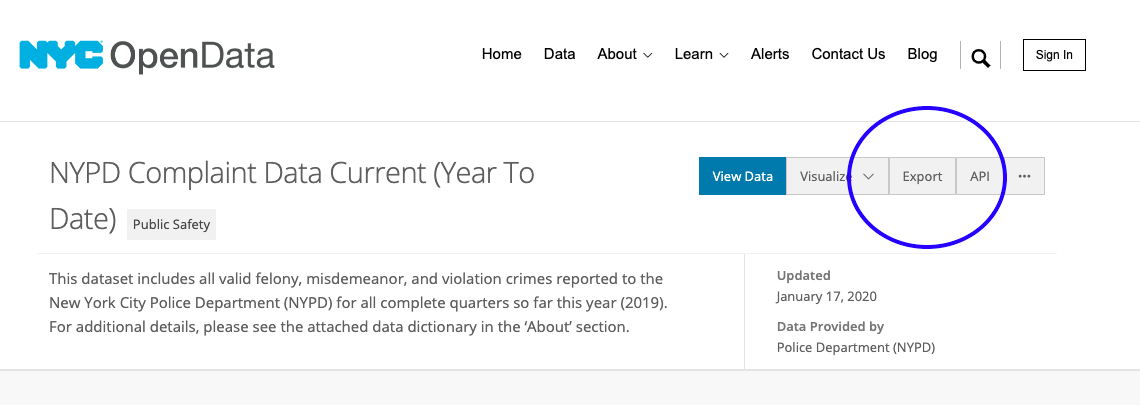
\includegraphics{images/NYPD_CD_main.png}
\caption{Location of Export button on the NYPD Complaint Data page of the NYC open data website}
\end{figure}

If you do this, however, you may end up with a very large file and this may slow things down in terms of download and processing time. For purposes of this first exercise, instead click the View Data button, as this will allow you to filter the data before downloading it:

\begin{figure}
\centering
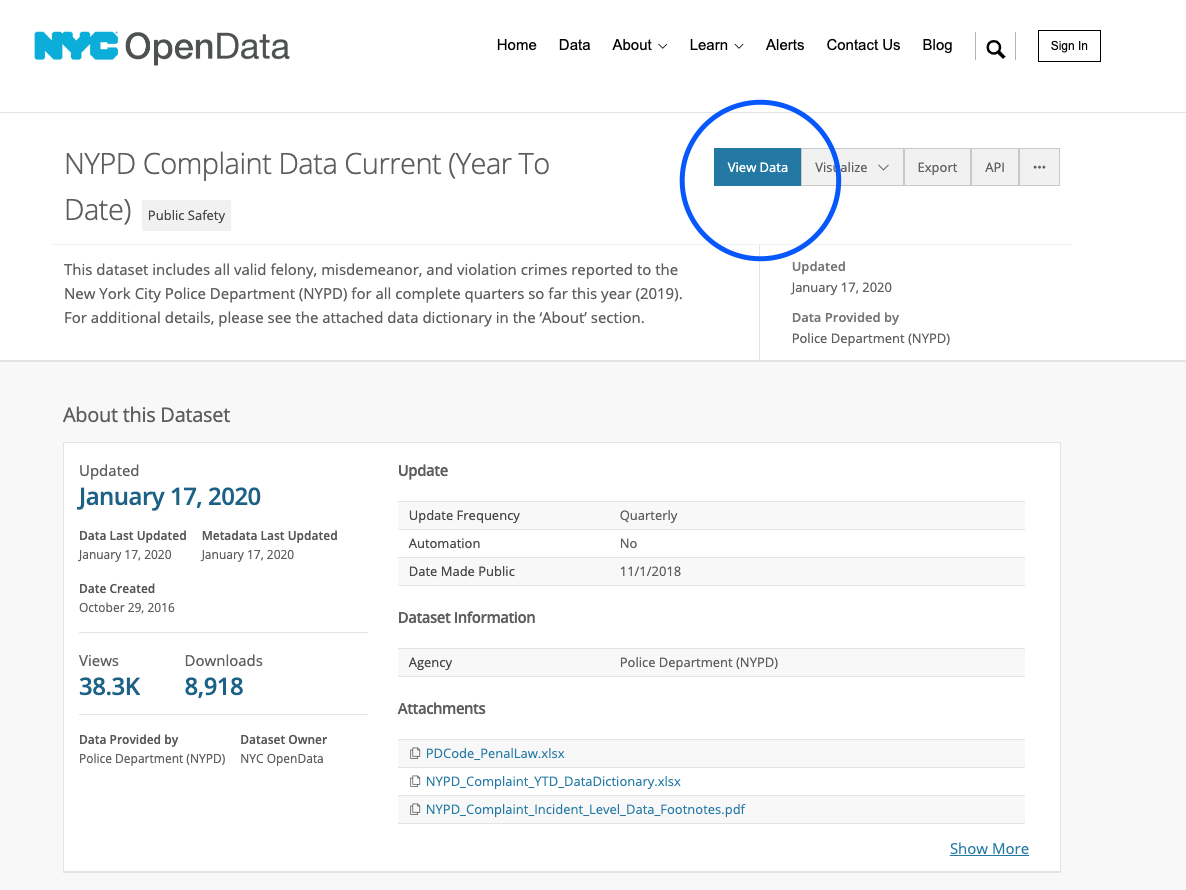
\includegraphics{images/NYPD_CD_view.png}
\caption{Location of the View Data button}
\end{figure}

Clicking on the View Data button will take you to a new page that includes a Filter button. Click on this and then click the Add a New Filter Condition button. You can easily filter the data by any of its fields (or by multiple fields). For this exercise, filter the OFNS\_DESC field (which is the description of the offense, as recorded by the NYPD) for FELONY ASSAULT:

\begin{figure}
\centering
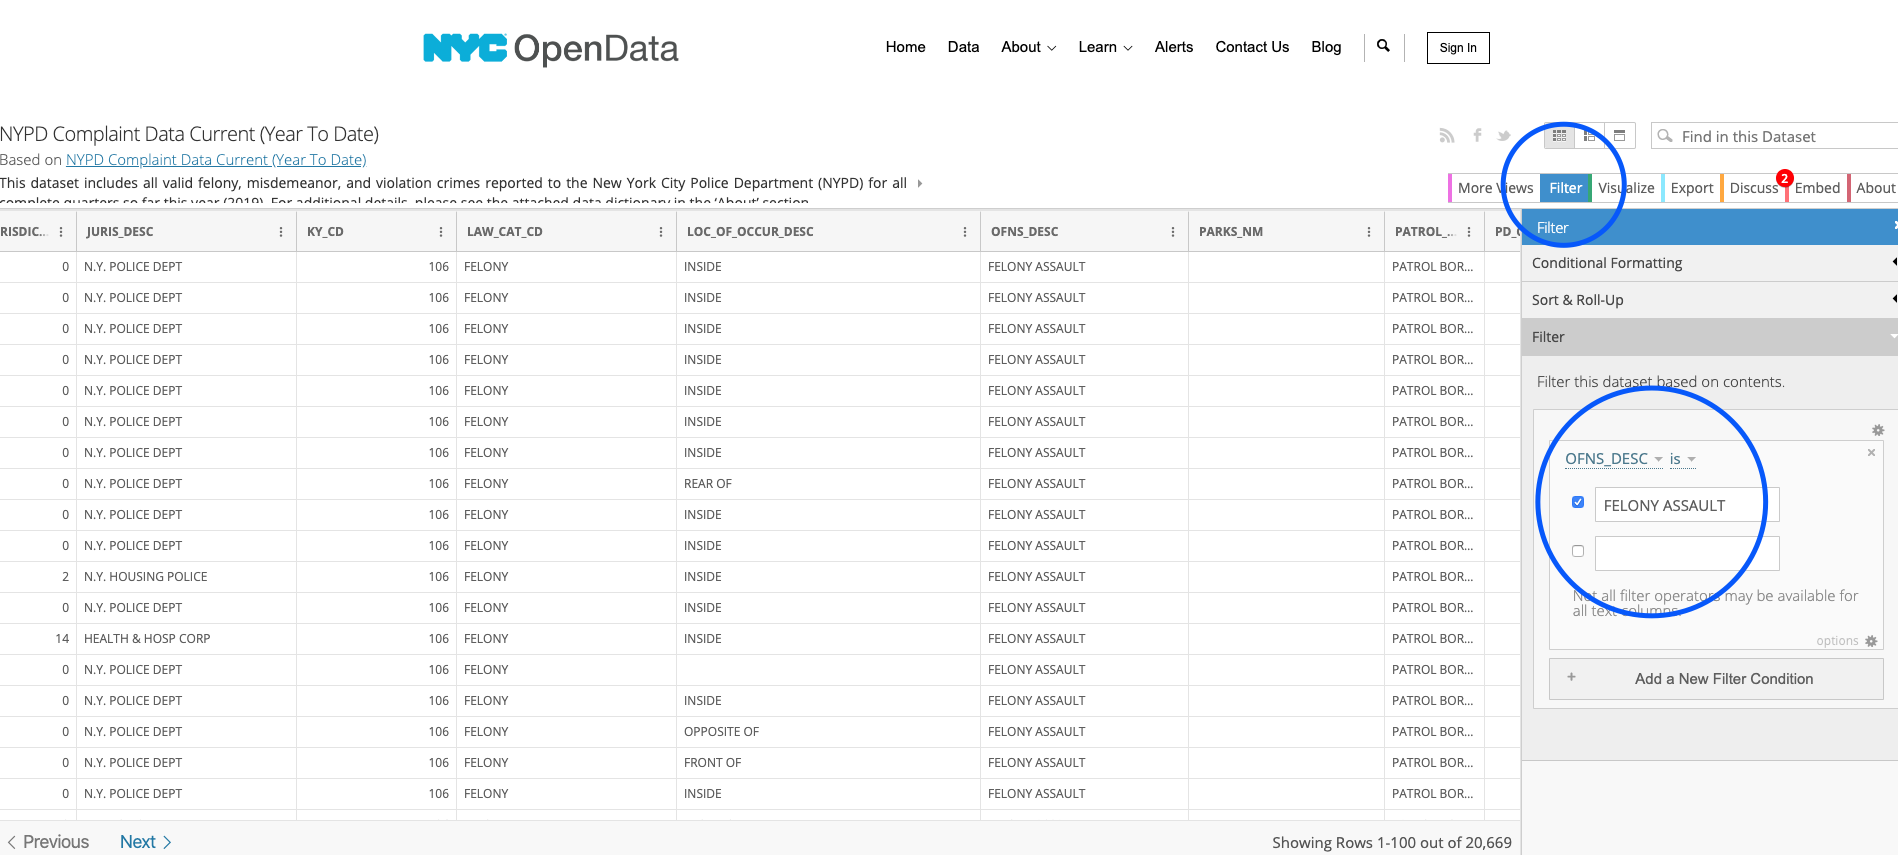
\includegraphics{images/NYPD_CD_filter.png}
\caption{Filtering the NYPD Complaint Data}
\end{figure}

Once you do this, you will see that the effect of the filter in the data displayed in the table on the left, incuding a large reduction in the number of records indicated at the bottom. Now export this filtered data using the Export button and selecting CSV as the format:

\begin{figure}
\centering
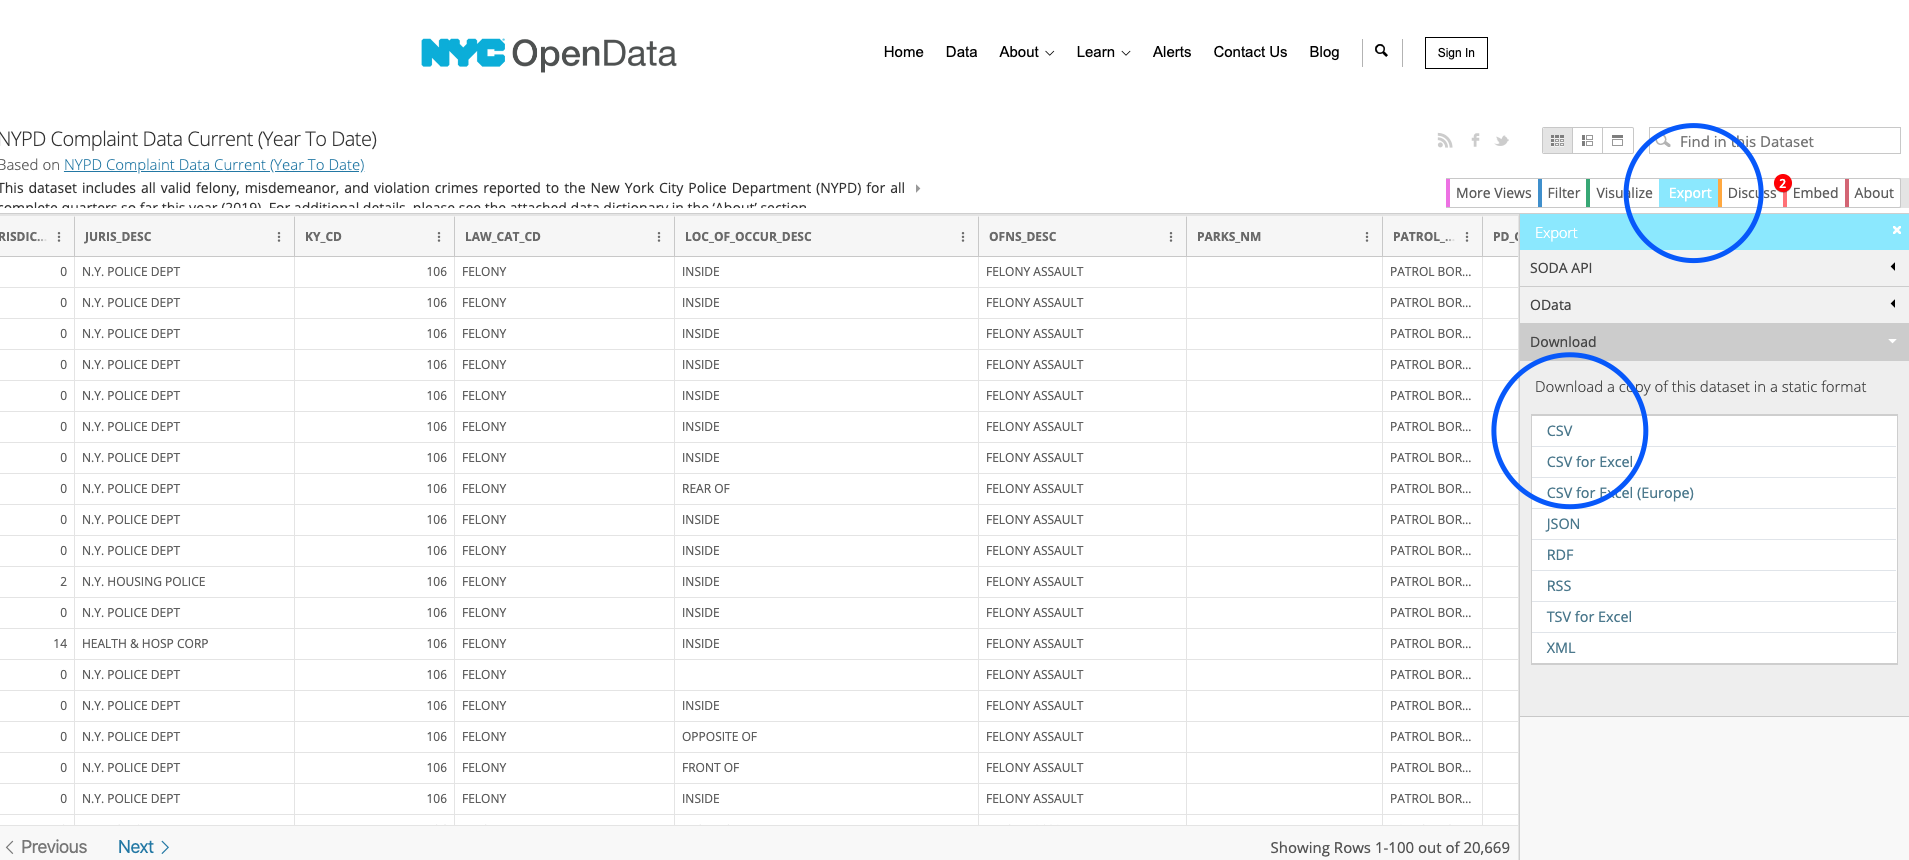
\includegraphics{images/NYPD_CD_visualize_export.png}
\caption{Exporting the NYPD Complaint data}
\end{figure}

Your browser will then let you choose a location to save the downloaded file. Remember this location so that you can find it in the next step and go ahead and complete the download.

\hypertarget{adding-data-to-your-map}{%
\subsection{Adding data to your map}\label{adding-data-to-your-map}}

Add the data to your map using Layer → Add Layer → Add Delimited Text Layer\ldots{}.

\begin{figure}
\centering
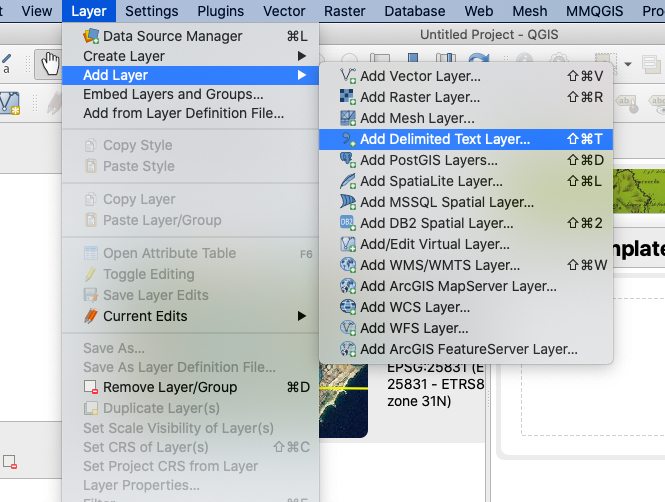
\includegraphics{images/add_deilmited_text_layer.png}
\caption{Screenshot of the Add Delimited Text Layer menu option in QGIS 3.10 for MacOS}
\end{figure}

In the dialog that comes up, click on the \ldots{} button to the right of the File name box at the top. Select the data file you just downloaded and saved.

\begin{figure}
\centering
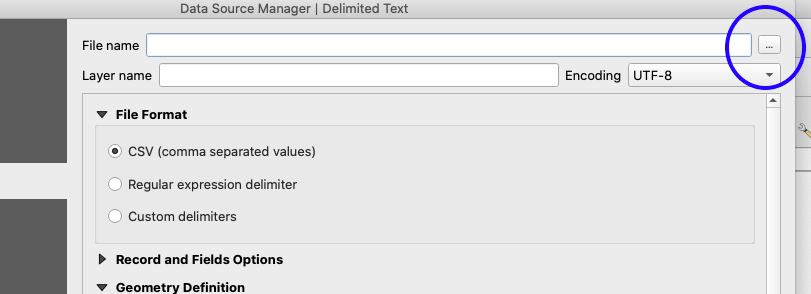
\includegraphics{images/add_delimited_file_chooser.png}
\caption{Choosing file in the dialog (botton at top right with bllue circle around it.)}
\end{figure}

Once you select the file in the dialog box, you will see that it is listed in the File name box. Note that you can also choose a Layer name. This is how the layer you are creating will be named on the layers bar of your QGIS interface. You will need to ensure that the proper File format is selected (in this case CSV) and you will need to provide information about geometry: In the Geometry definition box, make sure Point coordinates is selected. Make sure that the X field and Y field boxes contain the correct field names from your data for the x and y coordinates (in this case, the correct fields are Longitude and Latitute).

Now look at the Coordinate Reference System (CRS) selector, which is labelled Geometry CRS. This is a crucial setting because selecting the wrong CRS will lead to your layer being incorrectly placed on the map (or sometimes not visible at all). For points recorded as Latitude and Longitude, the correct CRS is EPSG 4326 - WGS 84, so make sure this is selected. We will talk more about other CRSs and how to determine which one your data relies on.

Note: Some of these settings may already be correctly set because QGIS automatically tries to figure them out from your file. So in many cases you will simply need to go through and double check them.

Once you have ensured that the settings are correct, look at the preview shown in the Sample Data section at the bottom of the window. You should see a table with data in rows and columns with headers. If you do not see this, go back and check the settings again.

Note: One common problem when importing CSV data is that QGIS may not be properly recognizing the character used to separate columns. CSV stands for comma-separated values, and in many systems this means that the columns are separated with commas (``,'') (as the name implies). In some systems, however, the default is to use semi-colons (``;'') instead of commas - and this is often the default on computers and software localized for Spain. Thus, for example, if you save an Excel sheet as a CSV file on a UPF lab computer, you may find that it is saved using semi-colons rather than commas. You can easily see whether it is commas or semi-colons (or something else) by simply opening your CSV file in a text editor and looking at it closely. If it is not a comma, you will need to specify which character it is by choosing the Custom delimiters setting and then either checking one of the preset boxes or simply typing in the character in the Others box.

Once you have finished with the settings, click the Add button at the bottom of the window.

\hypertarget{adding-data-using-an-api}{%
\subsection{Adding data using an API}\label{adding-data-using-an-api}}

We just added data by first downloading it to your computer because you will often need to work with data files in this way. Data providers, however, are increasingly making it possible to access their data sources using an Application Programming Interface (API). This can simply things for you, particularly when you will be working with a source frequently and will want the most updated data. We will discuss ways of working with APIs later on.

\hypertarget{working-with-multiple-layers}{%
\section{Working with Multiple Layers}\label{working-with-multiple-layers}}

When you first add the NYPD Complaint Data (or any other data source), you should be able to see it in the QGIS mapping window. Often, however, you will want to combine it with additional layers. For example, the NYPD Complaint Data will be much more useful it it is overlaid on top of a map of New York City. You can add such a map in many ways, but for now add Open Steet Map tiles using the instructions in Section \ref{osm-tiles}.

One issue you wil sometimes need to deal with is finding the features in a particular layer you have added. For example, if you have first added Open Street Map tiles and then added points, it may be that your map winder is focused on part of the world where there are no points. To view your new layer, you will need to pan and zoom to get to the location where it actually has data - in this case New York City. You can do that quickly by right-clicking on the layer in the Layers panel and selecting Zoom to Layer at the very top of the menu.

You may also need to make sure that the layer is not being covered by another layer. The order of the layers in the Layers Panel is the order in which they appear on the map (imagine actual layers of paper or transparent paper with features on a physical map). You can drag layers up and down in that list to change the order.

To learn more about each point marked on the map, select View → Identify Features and click on a point. You will see information in the Identify Results panel on the right (although you may need to expand that panel to see the values associated with each feature.

\hypertarget{printing-or-exporting-a-map}{%
\section{Printing or Exporting a Map}\label{printing-or-exporting-a-map}}

What you see in the QGIS console is useful for creating, modifying, and analyzing your map. If you want to share your map with someone or publish it as part of a report, you will want to use the print composer to produce high-quality output.

\hypertarget{setting-up-the-print-layout}{%
\subsection{Setting up the Print Layout}\label{setting-up-the-print-layout}}

Select Project → New Print Layout. In the dialog box that pops up, you can give this print layout a title or leave the box blank and click OK for the default title. You will now see a new window with a canvas that you can use to compose exactly how you want your map to look.

\hypertarget{adding-a-map}{%
\subsection{Adding a map}\label{adding-a-map}}

The most obvious thing you will want on your composed map is the map itself. Select Add Item → Add Map and then use the mouse to draw a rectangle on the canvas where you want the map to appear. Notice that the map that will now appear in that box is essentially a mirror image of the map you currently have in the main console (although the dimensions may be different depending on how you draw the box). After drawing the box, you can still move it around using the Edit → Select/Move Item tool, and you can move the map around within it using the Edit → Move Content tool. Notice that you can add more than one map to your canvas. This makes it possible to include inset maps, for example, showing where your detailed map lies at a larger scale.

\hypertarget{adding-a-scale-bar}{%
\subsection{Adding a scale bar}\label{adding-a-scale-bar}}

You may wish to add a scale bar to your map, and you can do this easily using Add Item → Add Scale Bar. Again, you will need to click on the map to position and resize the scale bar. You will notice that you also have many options to choose from in changing its appearance using the Item properties tab on the right.

\hypertarget{adding-a-legend}{%
\subsection{Adding a legend}\label{adding-a-legend}}

To add a legend, select Add Item → Add Legend and use the mouse to draw a rectangle where you want the legend to appear. The legend will be automatically filled with the information in your layers list, but you can modify this using the Item properties tab on the right. Select the legend you have added and scroll down the Item properties to the Legend Items section. Uncheck Auto update. Now select the layers you do not wish to see in the legend and click the minus sign at the bottom to remove them. Next click the item(s) that you want in the legend and use the editing button to edit the text that will appear. In the Main properties section you can also change the title and alignment of the legend text.

\hypertarget{exporting-your-map}{%
\subsection{Exporting your map}\label{exporting-your-map}}

When you are happy with your map, use Layout → Export as Image or Layout → Export as PDF or Layout → Export as SVG to export your map to a single file, which you can then share, embed in a report, or print.

\bibliography{book.bib,packages.bib}


\end{document}
